\documentclass[14pt]{article}
\usepackage{subfigure}
\usepackage{multicol}
\usepackage{graphicx}
\usepackage[utf8]{inputenc}
\usepackage[margin=.5in]{geometry}
\addtolength{\topmargin}{.875in}
\usepackage{xcolor}
\usepackage{titlesec}
\titleformat{\section}[block]{\color{black}\Large\bfseries\filcenter}{}{1em}{}

\begin{document}

\begin{centering}

\begin{multicols}{2}
\begin{description}
\item \Huge{Free Fall}
\item Toss
\end{description}
\end{multicols}

\begin{figure}[h!]
\begin{multicols}{2}
    \includegraphics[scale=0.6]{/Users/CoraJune/Documents/Github/Pozyx/new_models/freefall/figures/new_fitting/redBall.pdf}

    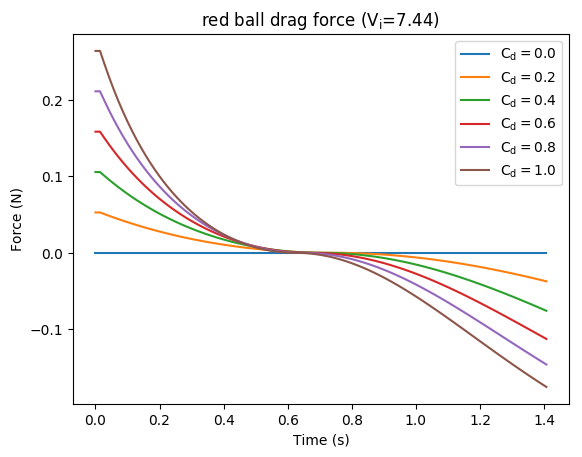
\includegraphics[scale=0.6]{/Users/CoraJune/Documents/Github/Pozyx/new_models/toss/figures/fitting/redBall.png}
\end{multicols}

\begin{multicols}{2}
    \includegraphics[scale=0.6]{/Users/CoraJune/Documents/Github/Pozyx/new_models/freefall/figures/accel_fitting/redBall.pdf}

    \includegraphics[scale=0.6]{/Users/CoraJune/Documents/Github/Pozyx/new_models/toss/figures/accel_fitting/redBall.pdf}
\end{multicols}

\end{figure}

\begin{figure}
\begin{multicols}{2}
    \includegraphics[scale=0.6]{/Users/CoraJune/Documents/Github/Pozyx/new_models/freefall/figures/new_fitting/yellowBall.pdf}

    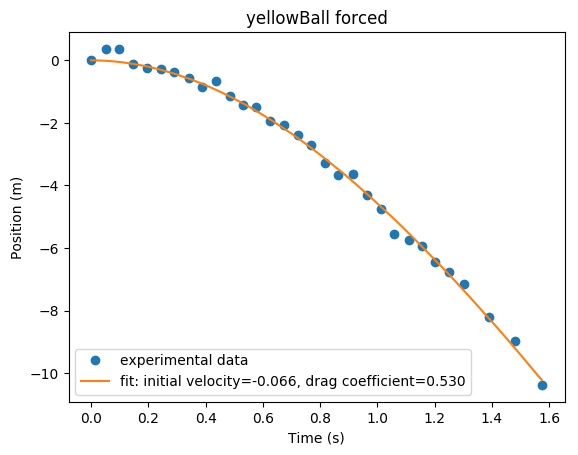
\includegraphics[scale=0.6]{/Users/CoraJune/Documents/Github/Pozyx/new_models/toss/figures/fitting/yellowBall.png}
\end{multicols}

\begin{multicols}{2}
    \includegraphics[scale=0.6]{/Users/CoraJune/Documents/Github/Pozyx/new_models/freefall/figures/accel_fitting/yellowBall.pdf}

    \includegraphics[scale=0.6]{/Users/CoraJune/Documents/Github/Pozyx/new_models/toss/figures/accel_fitting/yellowBall.pdf}
\end{multicols}

\end{figure}

\begin{figure}
\begin{multicols}{2}
    \includegraphics[scale=0.6]{/Users/CoraJune/Documents/Github/Pozyx/new_models/freefall/figures/new_fitting/blueBall.pdf}

    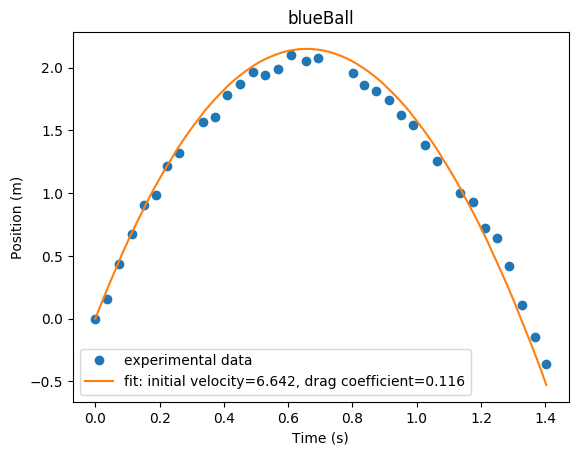
\includegraphics[scale=0.6]{/Users/CoraJune/Documents/Github/Pozyx/new_models/toss/figures/fitting/blueBall.png}
\end{multicols}

\begin{multicols}{2}
    \includegraphics[scale=0.6]{/Users/CoraJune/Documents/Github/Pozyx/new_models/freefall/figures/accel_fitting/blueBall.pdf}

    \includegraphics[scale=0.6]{/Users/CoraJune/Documents/Github/Pozyx/new_models/toss/figures/accel_fitting/blueBall.pdf}
\end{multicols}

\end{figure}

\begin{figure}
\begin{multicols}{2}
    \includegraphics[scale=0.6]{/Users/CoraJune/Documents/Github/Pozyx/new_models/freefall/figures/new_fitting/orangeBall.pdf}

    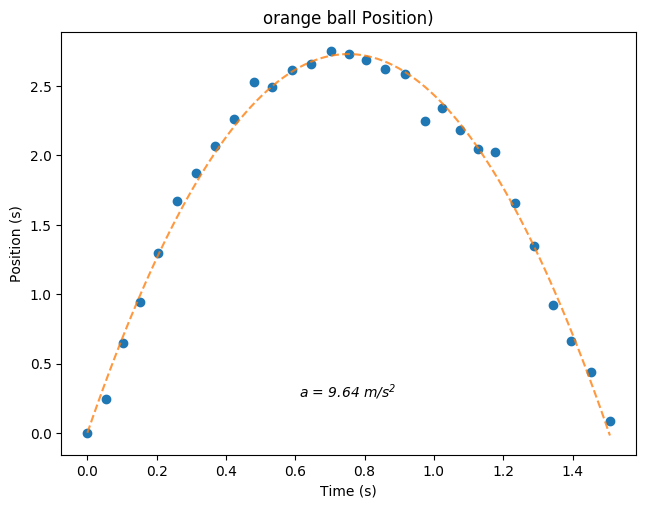
\includegraphics[scale=0.6]{/Users/CoraJune/Documents/Github/Pozyx/new_models/toss/figures/fitting/orangeBall.png}
\end{multicols}

\begin{multicols}{2}
    \includegraphics[scale=0.6]{/Users/CoraJune/Documents/Github/Pozyx/new_models/freefall/figures/accel_fitting/orangeBall.pdf}

    \includegraphics[scale=0.6]{/Users/CoraJune/Documents/Github/Pozyx/new_models/toss/figures/accel_fitting/orangeBall.pdf}
\end{multicols}

\end{figure}

\begin{figure}
\begin{multicols}{2}
    \includegraphics[scale=0.6]{/Users/CoraJune/Documents/Github/Pozyx/new_models/freefall/figures/new_fitting/rocket.pdf}

    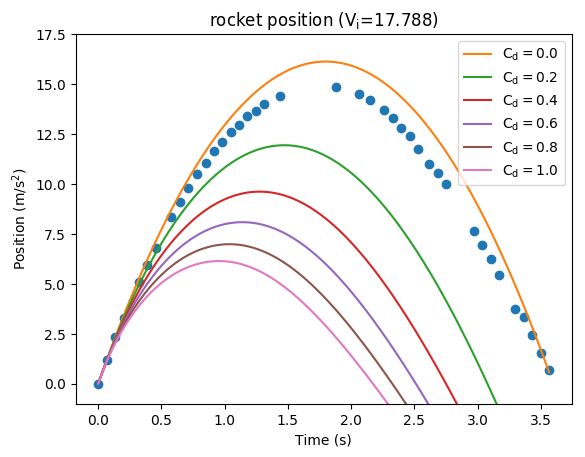
\includegraphics[scale=0.6]{/Users/CoraJune/Documents/Github/Pozyx/new_models/toss/figures/fitting/rocket.png}
\end{multicols}

\begin{multicols}{2}
    \includegraphics[scale=0.6]{/Users/CoraJune/Documents/Github/Pozyx/new_models/freefall/figures/accel_fitting/rocket.pdf}

    \includegraphics[scale=0.6]{/Users/CoraJune/Documents/Github/Pozyx/new_models/toss/figures/accel_fitting/rocket.pdf}
\end{multicols}

\end{figure}

\end{centering}
\end{document}
